\documentclass{article}
\usepackage{listings} % For code formatting
\usepackage[utf8]{inputenc}  % For encoding support
\usepackage{amsmath}         % For mathematical formatting
\usepackage{graphicx}        % For including images
\usepackage{xcolor}
\usepackage[a4paper, left=0.5in, right=0.5in, top=0.5in, bottom=0.5in]{geometry}  % Adjust margins here
\usepackage{tcolorbox}
\usepackage{palatino}  % Use Inconsolata font (or replace with your choice)
\usepackage{amsmath}
\usepackage{amssymb}
\usepackage{theorem}
\usepackage{tikz}
% Define colors
\definecolor{codebg}{RGB}{240, 240, 240}  % Light gray background
\definecolor{framecolor}{RGB}{100, 100, 100}  % Dark gray frame
\definecolor{titlebg}{RGB}{30, 30, 30}  % Dark title background
\definecolor{titlefg}{RGB}{255, 255, 255}  % White title text

% Custom lstset
\lstset{
    language=C++,                    
    basicstyle=\ttfamily\footnotesize\fontfamily{zi4}\selectfont, % Use Inconsolata
    keywordstyle=\bfseries\color{blue},        
    commentstyle=\itshape\color{gray},        
    stringstyle=\color{red},          
    numbers=left,                     
    numberstyle=\tiny\color{blue},    
    frame=single,                     
    breaklines=true,                   
    captionpos=b,                      
    backgroundcolor=\color{codebg},  % Light gray background
    rulecolor=\color{framecolor},    % Dark frame
    tabsize=4                         
}

% Custom command to add a styled heading
\newtcbox{\codebox}{colback=titlebg, colframe=titlebg, colupper=titlefg, 
  boxrule=0pt, arc=5pt, left=5pt, right=5pt, top=3pt, bottom=3pt}

\title{Parallel Programming Assignment 2 \\ Parallel Delta Stepping Algorithm Implementation and Experimentation using MPI}
\author{Ayush Raina, 22148}
\date{\today}

\begin{document}

\maketitle
\subsection*{Delta Stepping Algorithm}

Delta-Stepping is a parallel algorithm for solving the \textbf{Single-Source Shortest Path (SSSP)} problem, particularly effective on graphs with both \textbf{light} and \textbf{heavy} edges. It was introduced by Ulrich Meyer and Peter Sanders to achieve high performance on shared and distributed memory systems by exploiting parallelism in edge relaxation.

\subsubsection*{Problem Definition}
Given a graph \( G = (V, E) \), where \( V \) represents the set of vertices and \( E \) represents the set of weighted edges with non-negative weights, and a source vertex \( s \in V \), the objective of the algorithm is to compute the shortest path distance \( d(v) \) from the source \( s \) to every vertex \( v \in V \).

\subsubsection*{Key Concept: Light and Heavy Edges}
Edges are categorized based on a threshold parameter \( \Delta > 0 \):
\begin{itemize}
    \item \textbf{Light Edges}: Edges with weight \( w(e) \leq \Delta \)
    \item \textbf{Heavy Edges}: Edges with weight \( w(e) > \Delta \)
\end{itemize}

This distinction allows the algorithm to process light edges concurrently while deferring the processing of heavy edges, thereby enhancing parallel efficiency.

\subsubsection*{Algorithm Workflow}
\begin{enumerate}
    \item \textbf{Initialization:}
    \begin{itemize}
        \item Set the distance to the source vertex \( s \) as \( d(s) = 0 \), and to all other vertices as infinity \( d(v) = \infty \) for \( v \neq s \).
        \item Initialize a collection of buckets \( B[i] \), where each bucket stores vertices with distances in the range:
        \[
        B[i] = \{ v \mid i \times \Delta \leq d(v) < (i + 1) \times \Delta \}
        \]
    \end{itemize}
    
    \item \textbf{Bucket Processing Loop:}
    \begin{itemize}
        \item While there are non-empty buckets:
        \begin{itemize}
            \item Extract and process the \textbf{smallest non-empty bucket} \( B[i] \).
            \item Relax \textbf{light edges} of vertices in the bucket and update distances.
            \item Move vertices to appropriate future buckets based on updated distances.
        \end{itemize}
    \end{itemize}
    
    \item \textbf{Handling Heavy Edges:}
    \begin{itemize}
        \item After all light edges are processed, relax heavy edges.
        \item If the distance of a vertex changes, place it in the appropriate bucket.
    \end{itemize}
    
    \item \textbf{Termination:}
    \begin{itemize}
        \item The algorithm terminates when all buckets are empty, ensuring all shortest paths are computed.
    \end{itemize}
\end{enumerate}

\subsubsection*{Mathematical Formulation}
For a vertex \( v \) with current distance \( d(v) \), when relaxing an edge \( (v, u) \) with weight \( w \):

\[
  d(u) = \min(d(u), d(v) + w)
\]

If \( w \leq \Delta \), the edge is considered \textbf{light} and processed immediately. Otherwise, it is \textbf{heavy} and deferred.

\section*{Methodology}

\subsection*{Parallel Delta-Stepping Algorithm Implementation}

The parallel implementation of the Delta-Stepping algorithm aims to efficiently compute single-source shortest paths in weighted graphs by distributing computation across multiple processes using MPI (Message Passing Interface). This section details the key components, data structures, and methods used in our implementation.

\subsubsection*{Data Structures}

I have used the following user defined data structures to support the distributed computation:

\begin{itemize}
    \item \textbf{Edge}: A basic structure representing graph edges.
    \begin{verbatim}
    struct Edge {
        int Source;
        int Destination;
        int Weight;
    };
    \end{verbatim}
    
    \item \textbf{DistributedVertexMap}: Maps between global and local vertex IDs, essential for distributed processing.
    \begin{verbatim}
    struct DistributedVertexMap {
        unordered_map<int, int> LocalToGlobalMap;
        unordered_map<int, int> GlobalToLocalMap;
    };
    \end{verbatim}
    
    \item \textbf{VertexInfo}: Stores adjacency information for each vertex.
    \begin{verbatim}
    struct VertexInfo {
        vector<pair<int, int>> VertexEdges; // (destVertex, weight)
    };
    \end{verbatim}
    
    \item \textbf{VertexDistance}: Stores the current shortest path distance to a vertex.
    \begin{verbatim}
    struct VertexDistance {
        int distance;
    };
    \end{verbatim}
    
    \item \textbf{DistanceUpdate}: Structure for communicating distance updates between processes.
    \begin{verbatim}
    struct DistanceUpdate {
        int globalVertex;
        int newDistance;
    };
    \end{verbatim}
    
    \item \textbf{Buckets}: A vector of vectors where each inner vector contains vertices with similar tentative distances.
    \begin{verbatim}
    vector<vector<int>> buckets;
    \end{verbatim}
\end{itemize}

\subsubsection*{Communication Management}

Inter-process communication is handled by the \textbf{CommunicationBuffer} class, which:

\begin{itemize}
    \item Maintains a buffer of distance updates to be exchanged between processes
    \item Handles the transmission of updates using MPI
    \item Processes incoming updates and applies them to the local state
    \item Maintains consistency between distance values and bucket assignments
\end{itemize}

\begin{verbatim}
class CommunicationBuffer {
    // Stores pending distance updates
    vector<DistanceUpdate> updates;
    
    // References to shared data structures
    vector<VertexDistance>& LocalDistances;
    DistributedVertexMap& VertexMap;
    vector<vector<int>>& Buckets;
    int Delta;
    
    // Maps vertices to their current bucket
    unordered_map<int, int> vertexToBucketMap;
    
    // Methods for managing updates
    void addUpdate(int globalVertex, int newDistance);
    void SendUpdates(MPI_Comm comm, int DestinationRank);
    void ReceiveUpdates(MPI_Comm comm, int sourceRank);
    void ProcessAllUpdates(MPI_Comm comm);
};
\end{verbatim}

\subsubsection*{Algorithm Implementation}

The core algorithm is encapsulated in the \textbf{DeltaSteppingAlgorithm} class:

\begin{verbatim}
class DeltaSteppingAlgorithm {
    // References to data structures
    vector<VertexInfo>& localGraph;
    vector<VertexDistance>& localDistances;
    vector<vector<int>>& buckets;
    CommunicationBuffer& commBuffer;
    DistributedVertexMap& vertexMap;
    int delta;
    int rank;
    int size;
    MPI_Comm comm;
    
    // Performance metrics
    struct AlgorithmMetrics {
        int totalBucketsProcessed;
        int totalVerticesProcessed;
        int totalLightEdgesProcessed;
        int totalHeavyEdgesProcessed;
        int totalRelaxations;
        int totalCommunicationRounds;
    } metrics;
    
    // Methods
    void initializeBuckets();
    EdgeType classifyEdge(int weight);
    int findNextNonEmptyBucket(int startBucket);
    int findGlobalNextBucket(int localNextBucket, MPI_Comm comm);
    void relaxEdge(int sourceLocalIndex, int destGlobalVertex, int edgeWeight);
    void processLocalBuckets();
    void processLightEdges(int vertexIndex);
    void processHeavyEdges(int vertexIndex);
};
\end{verbatim}

\subsection*{Algorithm Phases}

The parallel Delta-Stepping algorithm execution involves several key phases:

\subsubsection*{Initialization}
\begin{enumerate}
    \item \textbf{Graph Distribution}: The input graph is read from a file and distributed among processes.
    \begin{verbatim}
    vector<Edge> globalGraph = parseGraphFile("SyntheticGraph.txt");
    DistributedVertexMap vertexMap = createVertexMapping(globalGraph, rank,
     numProcesses);
    vector<VertexInfo> localGraph = distributeGraph(globalGraph, rank, numProcesses,
     vertexMap);
    \end{verbatim}
    
    \item \textbf{Distance Initialization}: Distances are initialized (0 for source, infinity for others).
    \begin{verbatim}
    vector<VertexDistance> localDistances = initializeDistances(sourceVertex, vertexMap, rank);
    \end{verbatim}
    
    \item \textbf{Bucket Setup}: The source vertex is placed in bucket 0, and other structures are initialized.
    \begin{verbatim}
    vector<vector<int>> buckets;
    \end{verbatim}
\end{enumerate}

\subsubsection*{Main Processing Loop}
\begin{enumerate}
    \item \textbf{Finding Active Buckets}: Processes collaborate to identify the next bucket to process.
    \begin{verbatim}
    int localNextBucket = findNextNonEmptyBucket(currentBucketIndex);
    int globalNextBucket = findGlobalNextBucket(localNextBucket, comm);
    \end{verbatim}
    
    \item \textbf{Bucket Processing}: Each process processes vertices in the current bucket.
    \begin{verbatim}
    if (globalNextBucket < buckets.size() && !buckets[globalNextBucket].empty()) {
        vertices = std::move(buckets[globalNextBucket]);
        buckets[globalNextBucket].clear();
        
        // Process light edges first
        for (int vertex : vertices) {
            processLightEdges(vertex);
        }
        
        // Process heavy edges next
        for (int vertex : vertices) {
            processHeavyEdges(vertex);
        }
    }
    \end{verbatim}
    
    \item \textbf{Edge Classification and Relaxation}: 
    \begin{itemize}
        \item Light edges (weight $\leq \delta$) are processed first.
        \item Heavy edges (weight $> \delta$) are processed after light edges.
        \item Edge relaxation may update distances and bucket assignments.
    \end{itemize}
    \begin{verbatim}
    EdgeType classifyEdge(int weight) {
        return (weight <= delta) ? Light : Heavy;
    }
    
    void relaxEdge(int sourceLocalIndex, int destGlobalVertex, int edgeWeight) {
        int currentDistance = localDistances[sourceLocalIndex].distance;
        if (currentDistance == numeric_limits<int>::max())
            return;
            
        int newDistance = currentDistance + edgeWeight;
        // Update distances if better path found
        // ...
    }
    \end{verbatim}
    
    \item \textbf{Communication and Synchronization}: After processing, processes exchange distance updates.
    \begin{verbatim}
    commBuffer.ProcessAllUpdates(comm);
    \end{verbatim}
\end{enumerate}

\subsubsection*{Result Collection and Performance Measurement}
\begin{enumerate}
    \item \textbf{Timer Implementation}: Performance is measured using MPI timing functions.
    \begin{verbatim}
    double StartTime = MPI_Wtime();
    // Algorithm execution
    double EndTime = MPI_Wtime();
    double elapsedTime = EndTime - StartTime;
    \end{verbatim}
    
    \item \textbf{Performance Metrics}: Several metrics are collected for analysis.
    \begin{verbatim}
    struct AlgorithmMetrics {
        int totalBucketsProcessed = 0;
        int totalVerticesProcessed = 0;
        int totalLightEdgesProcessed = 0;
        int totalHeavyEdgesProcessed = 0;
        int totalRelaxations = 0;
        int totalCommunicationRounds = 0;
    } metrics;
    \end{verbatim}
    
    \item \textbf{Result Aggregation}: Final results are collected from all processes to rank 0.
    \begin{verbatim}
    gatherAndSaveFinalResults(localDistances, vertexMap, sourceVertex, comm);
    \end{verbatim}
\end{enumerate}

\subsection*{Key Implementation Considerations}

\subsubsection*{Load Balancing}
Vertices are distributed among processes using a modulo-based approach, where vertex $v$ is assigned to process $v \bmod p$ (where $p$ is the number of processes). This simple scheme aims to balance the computational load.

\subsubsection*{Delta Parameter}
The $\delta$ parameter (set to 1 in our implementation) determines the bucket size and influences:
\begin{itemize}
    \item Edge classification into light and heavy edges
    \item Granularity of parallel execution
    \item Communication frequency between processes
\end{itemize}

\subsubsection*{Termination Condition}
The algorithm terminates when no process has more vertices to process, detected through a collective operation:
\begin{verbatim}
int hasMoreWork = (localNextBucket != -1) ? 1 : 0;
int totalWork = 0;
MPI_Allreduce(&hasMoreWork, &totalWork, 1, MPI_INT, MPI_SUM, comm);
if (totalWork == 0) {
    // Algorithm terminates
    break;
}
\end{verbatim}

\subsection*{Verification and Validation}
The implementation includes functions to:
\begin{itemize}
    \item Verify correct graph distribution across processes
    \item Validate results by comparing against sequential Dijkstra's algorithm output
    \item Collect and analyze performance metrics
\end{itemize}

\begin{verbatim}
bool isResultMatch = compareOutputFiles("dijkstra_output.txt", 
                                       "ParallelDeltaSteppingOutput.txt");
\end{verbatim}

\subsection*{Experimental Setup}
All the experiments are done on teaching cluster provided to us. The graph used in experiementation contains 1,971,281 vertices and 5,533,214 edges with randomly assigned weights $w(e) \in [1, 100]$. We are choosing source vertex to be 0. Following is the execution times for 1,2,4,8,16,32,64 processors along with Speedup and Efficiency for different Delta Values

\begin{table}[h]
    \centering
    \begin{tabular}{|c|c|c|c|c|c|c|c|c|}
        \hline
        \textbf{Delta} & \textbf{1 Proc} & \textbf{2 Proc} & \textbf{4 Proc} & \textbf{8 Proc} & \textbf{16 Proc} & \textbf{32 Proc} & \textbf{64 Proc} \\
        \hline
        1   & 4.503  & 3.515  & 3.100  & 3.026  & 2.939  & 3.467 & 8.079 \\
        5  & 4.536  & 3.523  & 3.091  & 2.825  & 2.947   & 3.399   & 8.108      \\
        10  & 4.530  & 3.631  & 3.090  & 2.908  & 3.053   & 3.412   & 7.903    \\
        20  & 4.507  & 3.536  & 3.042 & 2.892   & 2.990  & 3.421 & 8.117   \\
        30 & 4.493  & 3.619  & 3.121  & 2.942  & 2.983   & 3.434   & 7.930  \\
        40 & 4.500   & 3.525  & 3.120  & 2.938  & 2.973   & 3.490   & 8.353  \\
        50 & 4.504   & 3.538  & 3.186  & 2.965  & 3.000   & 3.420   & 7.992     \\
        60 & 4.507   & 3.516  & 3.185  & 2.928  & 2.916   & 3.583   & 8.651    \\
        70 & 4.498   & 3.455  & 3.096  & 2.877  & 2.971   & 3.563   & 8.428    \\
        80 & 4.536   & 3.459  & 3.064  & 3.042  & 2.922   & 4.855   & 8.156   \\
        90 & 4.505   & 3.440  & 3.259  & 3.032  & 2.945   & 3.570   & 8.059    \\
        100 & 4.511  & 3.543  & 3.148  & 2.955  & 2.964   & 3.376   & 8.425      \\
        \hline
    \end{tabular}
    \caption{Execution times (in seconds) for different processor counts and Delta values}
    \label{tab:execution_times}
\end{table}

In the above table, the execution time for involving more than 1 processor is reported for the processor which took the maximum time. Here are some plots to visualize the above data.

\begin{figure}[h]
    \centering
    \includegraphics[width=0.8\textwidth]{speedup.png}
    \caption{Speedup vs Number of Processors for Different Delta Values}
    \label{fig:speedup}
\end{figure}

\begin{figure}[h]
    \centering
    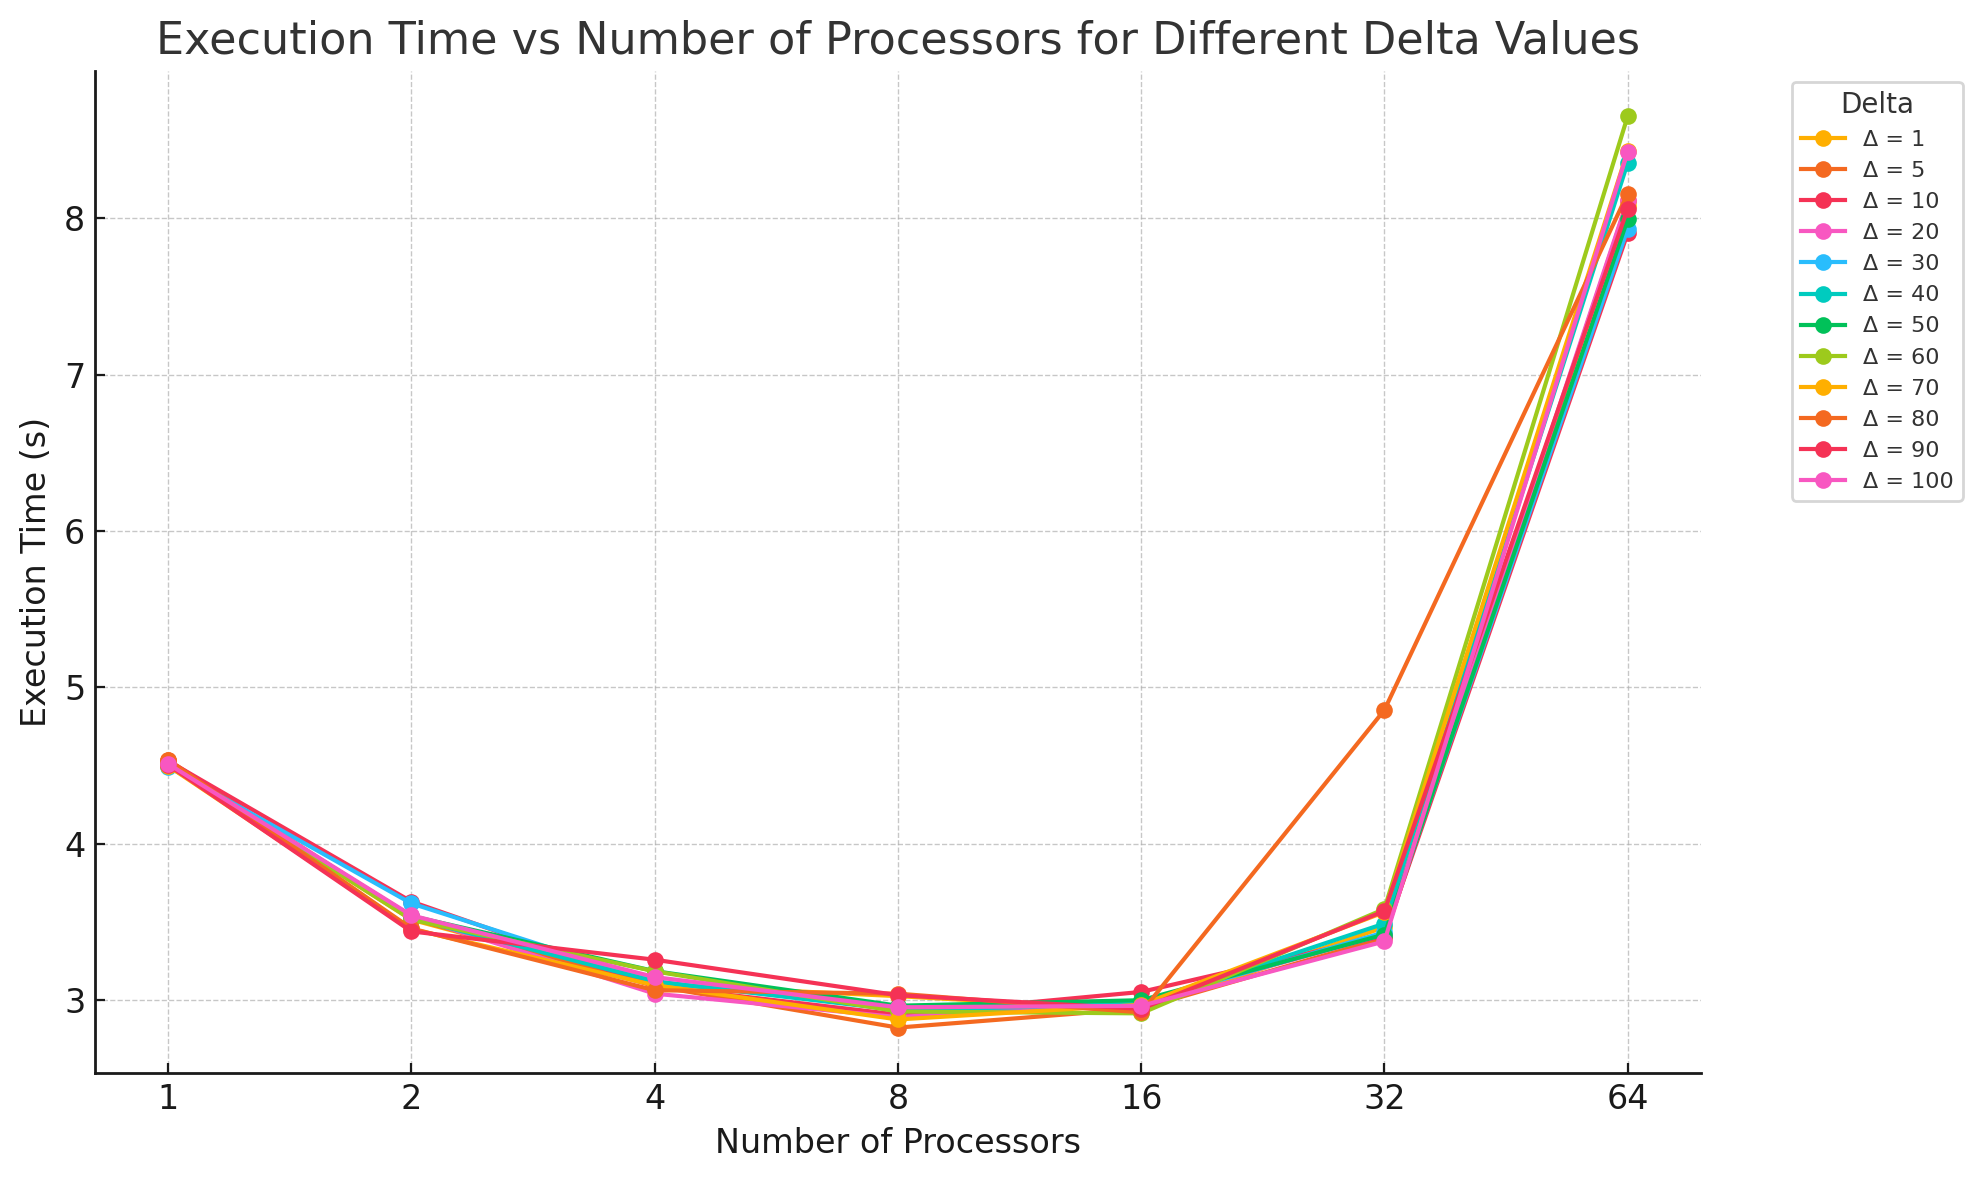
\includegraphics[width=0.8\textwidth]{executionTime.png}
    \caption{Execution Time vs Number of Processors for Different Delta Values}
    \label{fig:efficiency}
\end{figure}

\newpage

\subsection*{Parallel Overhead Calculation}
We can also calculate Parallel Overhead which quantifies extra work incurred due to parallelization - such as communication, synchronization and load imbalance. It is defined as $PO = T_N \times P - T_1$ where $T_N$ is the execution time for N processors and $T_1$ is the execution time for 1 processor. Here is the plot for Parallel Overhead for different Delta Values.

\begin{figure}[h]
    \centering
    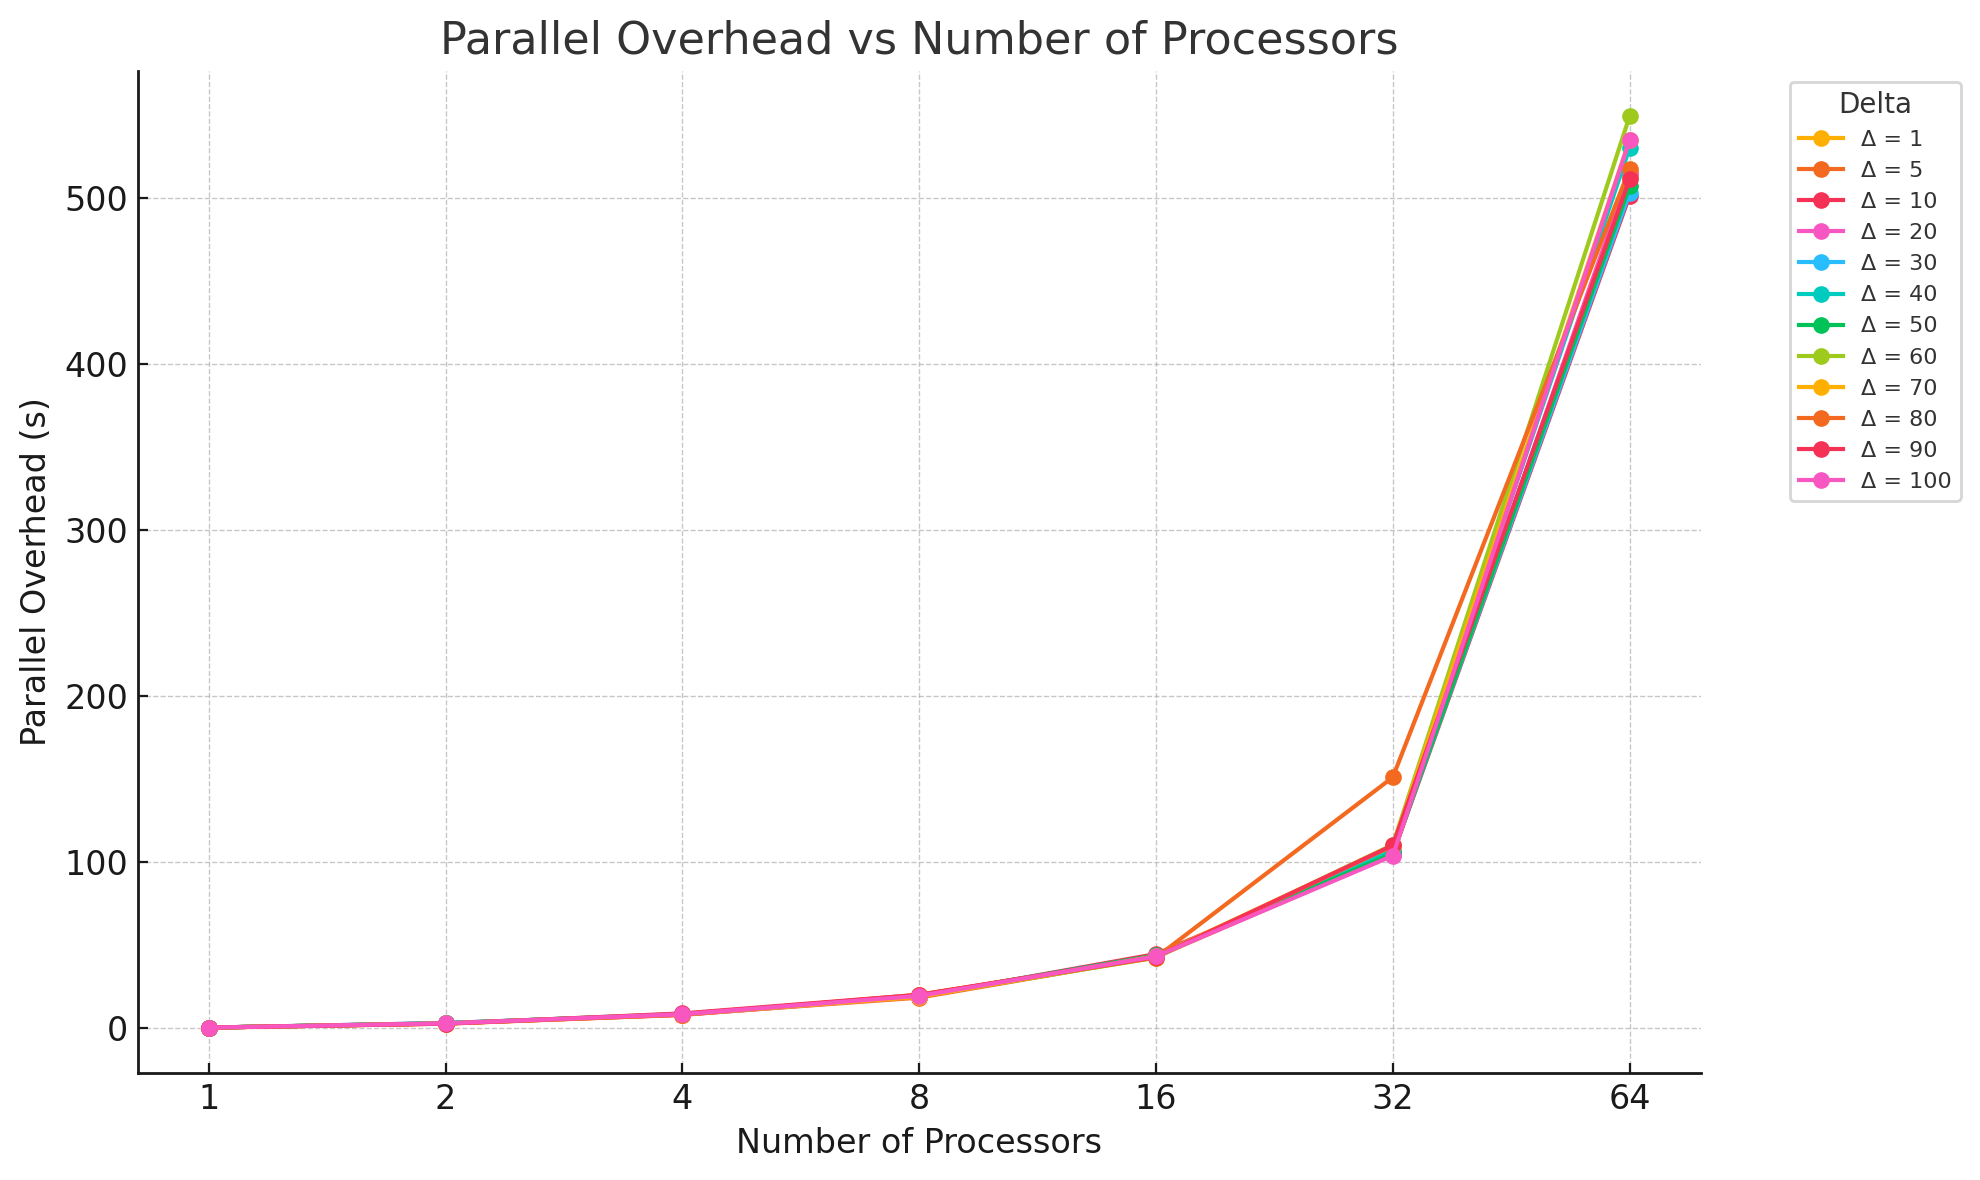
\includegraphics[width=0.8\textwidth]{overhead.png}
    \caption{Parallel Overhead vs Number of Processors for Different Delta Values}
    \label{fig:parallelOverhead}
\end{figure}

One more reason, I think for huge increase in overhead when we move to 64 processor from 32 processors is because the machine in which we are running the code has 32 cores. I tried all these experiments with my 24 core machine also in which same pattern followed. Initially execution time kept decreasing until 16 cores, then if I use \textbf{--oversubscribe} flag to run with 32 and 64 processors, the execution time increased. 

\newpage 

Here is efficiency plot for different Delta Values.
\begin{figure}[h]
    \centering
    \includegraphics[width=0.8\textwidth]{efficiency.png}
    \caption{Efficiency vs Number of Processors for Different Delta Values}
    \label{fig:efficiency}
\end{figure}

From above plot we can see that even we are lowering the execution time till 8 processors, but still the resource utilization is not up to the mark. This is because of communication overheads, synchronization overheads as Delta Stepping Algorithm is a bulk synchronization algorithm, and non trivial programming using MPI. My implementation is around 1000 lines of code and I used \textbf{modulus} operator to distribute the vertices among processors, due to which all processors have got almost equal number of vertices to process. So \textbf{load imbalance} is not an issue, \textbf{communication and synchronization overheads} are the main reasons for low efficiency.


\section*{Hybrid CPU-GPU Implementation Methodology}

Our hybrid implementation combines CUDA for GPU-accelerated edge relaxation with CPU-based bucket management to achieve high-performance shortest path computation. This section details the design, data structures, and algorithms used in our CUDA-based Delta-Stepping implementation.

\subsection*{System Architecture}

The implementation follows a heterogeneous computing model:
\begin{itemize}
    \item \textbf{CPU}: Manages algorithm control flow, bucket processing, and data orchestration
    \item \textbf{GPU}: Accelerates the computationally intensive edge relaxation operations through CUDA kernels
\end{itemize}

\subsection*{Data Structures}

\subsubsection*{Graph Representation}
The graph is stored in multiple formats to optimize different operations:

\begin{verbatim}
struct Graph {
    int num_nodes = 0;
    int num_edges = 0;
    vector<vector<pair<int, int>>> adj_list; // [node] -> list of (dest, weight)
    vector<int> src, dst, weight; // Edge list for CUDA
};
\end{verbatim}

\begin{itemize}
    \item \textbf{Adjacency List}: Traditional representation for CPU operations
    \item \textbf{Edge List Arrays}: Three parallel arrays (source, destination, weight) optimized for GPU memory access patterns
\end{itemize}

\subsubsection*{Distance Array}
A single array tracks the tentative shortest distance to each node:
\begin{verbatim}
vector<int> dist(num_nodes, DIST_INF);
\end{verbatim}

\subsubsection*{Bucket Structure}
Buckets are implemented as a vector of sets, where each set contains vertices with distances in a specific range:
\begin{verbatim}
const int MAX_BUCKET_COUNT = 1000;
vector<set<int>> buckets(MAX_BUCKET_COUNT);
\end{verbatim}

\subsubsection*{Performance Metrics}
A dedicated structure collects various algorithm performance metrics:
\begin{verbatim}
struct PerformanceMetrics {
    double total_time_seconds;
    int iteration_count;
    vector<double> per_bucket_time;
    vector<int> bucket_sizes;
    double data_transfer_time;
    double kernel_execution_time;
    double bucket_processing_time;
};
\end{verbatim}

\subsection*{GPU Kernel Design}

The core of the computation is performed by the CUDA kernel that relaxes edges for vertices in the current bucket:

\begin{verbatim}
__global__ void relaxEdgesKernel(
    int* d_edges_src, int* d_edges_dst, int* d_edges_weight, int num_edges,
    int* d_dist, bool* d_changed, int* d_bucket_nodes, int num_bucket_nodes,
    int delta, int current_bucket) {
    
    int idx = blockIdx.x * blockDim.x + threadIdx.x;
    
    if (idx < num_bucket_nodes) {
        int node = d_bucket_nodes[idx];
        
        // Only process if the node's distance is valid
        if (d_dist[node] != DIST_INF) {
            // Iterate through edges
            for (int e = 0; e < num_edges; e++) {
                if (d_edges_src[e] == node) {
                    int v = d_edges_dst[e];
                    int w = d_edges_weight[e];
                    
                    // Calculate new distance
                    int new_dist = d_dist[node] + w;
                    
                    // Check for overflow and only update if new_dist is less
                    if (new_dist >= 0 && (d_dist[v] == DIST_INF || new_dist < d_dist[v])) {
                        atomicMin(&d_dist[v], new_dist);
                        *d_changed = true;
                    }
                }
            }
        }
    }
}
\end{verbatim}

Key features of the kernel:
\begin{itemize}
    \item \textbf{Thread Structure}: Each thread processes a single vertex from the current bucket
    \item \textbf{Atomic Operations}: Uses \texttt{atomicMin()} to safely update distances in parallel
    \item \textbf{Change Detection}: Sets a global flag when any distance is updated
    \item \textbf{Edge Traversal}: Searches through all edges to find those originating from the current node
\end{itemize}

\subsection*{Algorithm Implementation}

The hybrid Delta-Stepping algorithm follows these key steps:

\subsubsection*{Initialization Phase}
\begin{enumerate}
    \item \textbf{Graph Loading}: Read graph from file into memory
    \begin{verbatim}
    Graph graph = readGraph("SyntheticGraph.txt");
    \end{verbatim}
    
    \item \textbf{Distance Array Initialization}: Set source node distance to 0, all others to infinity
    \begin{verbatim}
    vector<int> dist(num_nodes, DIST_INF);
    dist[source] = 0;
    \end{verbatim}
    
    \item \textbf{Bucket Initialization}: Place source node in bucket 0
    \begin{verbatim}
    buckets[0].insert(source);
    \end{verbatim}
    
    \item \textbf{GPU Memory Allocation}: Allocate and initialize device memory
    \begin{verbatim}
    checkCudaError(cudaMalloc(&d_edges_src, num_edges * sizeof(int)),
     "allocate d_edges_src");
    checkCudaError(cudaMalloc(&d_edges_dst, num_edges * sizeof(int)),
     "allocate d_edges_dst");
    checkCudaError(cudaMalloc(&d_edges_weight, num_edges * sizeof(int)), 
    "allocate d_edges_weight");
    checkCudaError(cudaMalloc(&d_dist, num_nodes * sizeof(int)),
     "allocate d_dist");
    checkCudaError(cudaMalloc(&d_changed, sizeof(bool)),
     "allocate d_changed");
    checkCudaError(cudaMalloc(&d_bucket_nodes, num_nodes * sizeof(int)), 
    "allocate d_bucket_nodes");
    \end{verbatim}
    
    \item \textbf{Data Transfer to GPU}: Copy graph structure and initial distances to GPU memory
    \begin{verbatim}
    checkCudaError(cudaMemcpy(d_edges_src, graph.src.data(), num_edges * sizeof(int), 
                              cudaMemcpyHostToDevice), "copy edges_src");
    checkCudaError(cudaMemcpy(d_edges_dst, graph.dst.data(), num_edges * sizeof(int), 
                              cudaMemcpyHostToDevice), "copy edges_dst");
    checkCudaError(cudaMemcpy(d_edges_weight, graph.weight.data(),
     num_edges * sizeof(int), cudaMemcpyHostToDevice), "copy edges_weight");
    checkCudaError(cudaMemcpy(d_dist, dist.data(), num_nodes * sizeof(int), 
                              cudaMemcpyHostToDevice), "copy initial dist");
    \end{verbatim}
\end{enumerate}

\subsubsection*{Main Processing Loop}
\begin{enumerate}
    \item \textbf{Bucket Selection}: Find the smallest non-empty bucket
    \begin{verbatim}
    int smallest_bucket = -1;
    for (int b = current_bucket; b < buckets.size(); b++) {
        if (!buckets[b].empty()) {
            smallest_bucket = b;
            break;
        }
    }
    \end{verbatim}
    
    \item \textbf{Bucket Extraction}: Move nodes from current bucket to a working set
    \begin{verbatim}
    vector<int> bucket_nodes(buckets[smallest_bucket].begin(),
     buckets[smallest_bucket].end());
    buckets[smallest_bucket].clear();
    \end{verbatim}
    
    \item \textbf{Kernel Preparation}: Copy current bucket nodes to GPU
    \begin{verbatim}
    checkCudaError(cudaMemcpy(d_bucket_nodes, bucket_nodes.data(), 
                              bucket_nodes.size() * sizeof(int), 
                              cudaMemcpyHostToDevice), "copy bucket nodes");
    \end{verbatim}
    
    \item \textbf{Kernel Execution}: Launch CUDA kernel to relax edges
    \begin{verbatim}
    int threadsPerBlock = 256;
    int blocksPerGrid = (bucket_nodes.size() + threadsPerBlock - 1) / threadsPerBlock;
    
    relaxEdgesKernel<<<blocksPerGrid, threadsPerBlock>>>(
        d_edges_src, d_edges_dst, d_edges_weight, num_edges,
        d_dist, d_changed, d_bucket_nodes, bucket_nodes.size(),
        delta, smallest_bucket
    );
    \end{verbatim}
    
    \item \textbf{Result Retrieval}: Copy updated distances and change flag back from GPU
    \begin{verbatim}
    checkCudaError(cudaMemcpy(&changed, d_changed, sizeof(bool), 
                              cudaMemcpyDeviceToHost), "copy changed flag");
    checkCudaError(cudaMemcpy(dist.data(), d_dist, num_nodes * sizeof(int), 
                              cudaMemcpyDeviceToHost), "copy distances");
    \end{verbatim}
    
    \item \textbf{Bucket Update}: Reassign nodes to buckets based on updated distances
    \begin{verbatim}
    if (changed) {
        for (int i = 0; i < num_nodes; i++) {
            // If distance was updated and is now finite
            if (dist[i] != DIST_INF) {
                int bucket_id = dist[i] / delta;
                
                // Only insert if not already processed in current iteration
                if (i != source && find(bucket_nodes.begin(), bucket_nodes.end(), i)
                 == bucket_nodes.end()) {
                    buckets[bucket_id].insert(i);
                }
            }
        }
    }
    \end{verbatim}
\end{enumerate}

\subsubsection*{Termination and Results}
\begin{enumerate}
    \item \textbf{Algorithm Termination}: The algorithm terminates when either:
    \begin{itemize}
        \item No more non-empty buckets exist
        \item No distance updates were made in the last iteration
        \item Maximum iteration count is reached (safety measure)
    \end{itemize}
    
    \item \textbf{Resource Cleanup}: Free GPU memory
    \begin{verbatim}
    cudaFree(d_edges_src);
    cudaFree(d_edges_dst);
    cudaFree(d_edges_weight);
    cudaFree(d_dist);
    cudaFree(d_changed);
    cudaFree(d_bucket_nodes);
    \end{verbatim}
    
    \item \textbf{Result Validation}: Compare results with sequential Dijkstra implementation
    \begin{verbatim}
    bool isResultMatch = compareOutputFiles("dijkstra_output.txt", 
                                           "HybridDeltaSteppingResults.txt");
    \end{verbatim}
\end{enumerate}

\subsection*{Performance Analysis}

Several performance metrics are collected during the algorithm execution:

\subsubsection*{Timing Metrics}
\begin{itemize}
    \item \textbf{Total Execution Time}: End-to-end runtime of the algorithm
    \item \textbf{Data Transfer Time}: Time spent transferring data between CPU and GPU
    \item \textbf{Kernel Execution Time}: Time spent in GPU computation
    \item \textbf{Per-Bucket Processing Time}: Processing time for each individual bucket
\end{itemize}

\section*{Experimental Results}

We implemented the same Delta Stepping Algorithm using Open MP and CUDA. We used Open MP for parallelizing the bucket processing loop and CUDA for parallelizing the edge relaxation step. We used 8 threads for Open MP and 256 threads per block for CUDA.Here is the execution times for different Delta Values.

\begin{table}[ht]
    \centering
    \caption{Execution Times for Different Delta Values (OpenMP + CUDA)}
    \begin{tabular}{|c|c|}
        \hline
        \textbf{Delta Value} & \textbf{Execution Time (s)} \\
        \hline
        1 & 6.1021 \\
        \hline
        5 & 3.4281 \\
        \hline
        10 & 3.3989 \\
        \hline
        20 & 1.5955 \\
        \hline
        30 & 2.4969 \\
        \hline
        40 & 1.5924 \\
        \hline
        50 & 1.3124 \\
        \hline
        60 & 1.3066 \\
        \hline
        70 & 1.61707 \\
        \hline
        80 & 1.5882 \\
        \hline
        90 & 2.2041 \\
        \hline
        100 & 1.3141 \\
        \hline
    \end{tabular}
    \label{tab:delta_timing}

    Assuming Sequential Execution Time (T\_seq): 4.503 seconds
    \begin{equation}
        \text{Speedup} = \frac{T_{seq}}{T_{par}}
    \end{equation}
    and 
    \begin{equation}
        \text{Efficiency} = \frac{\text{Speedup}}{P}
    \end{equation}
    Where $T_{par}$ is the execution time for parallel implementation and $P$ is the number of processors which is 8 in this case.

\end{table}
Here are the plots for speedup, execution times and efficiency for OpenMP + CUDA implementation for different Delta Values.

\begin{figure}[h]
    \centering
    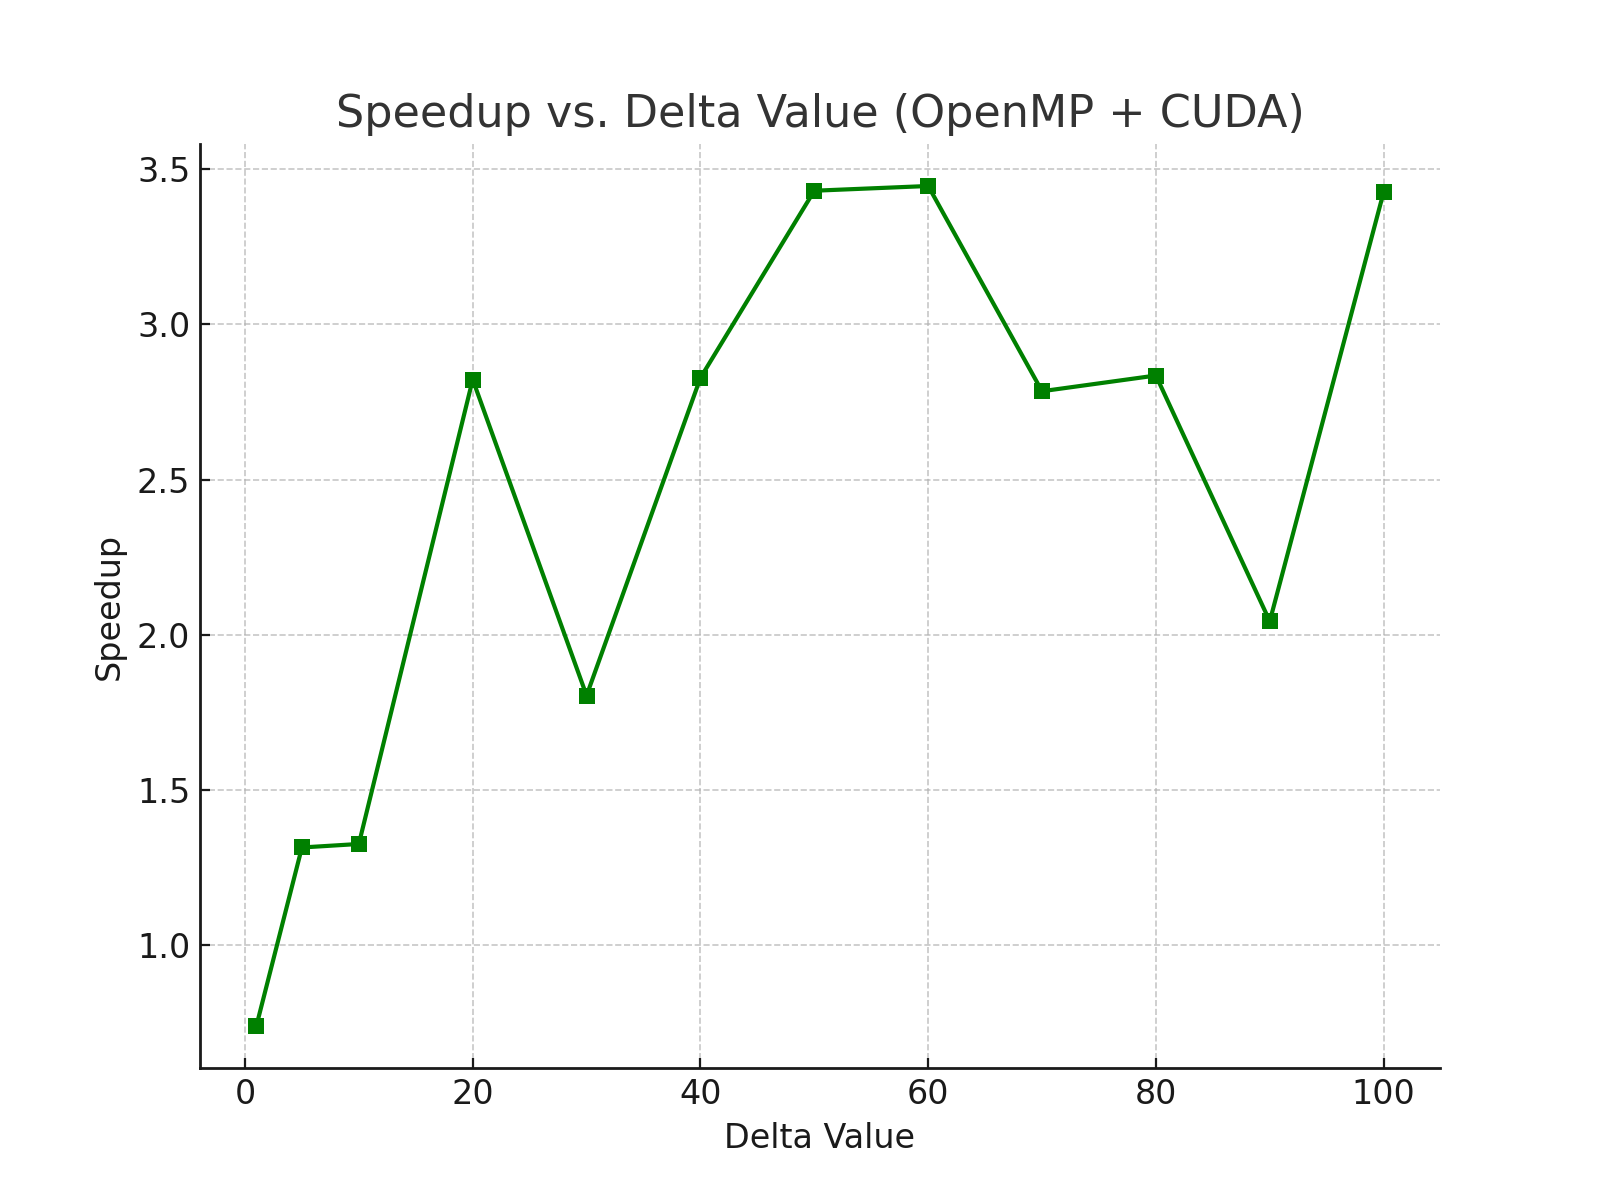
\includegraphics[width=0.4\textwidth]{speedup_vs_delta.png}
    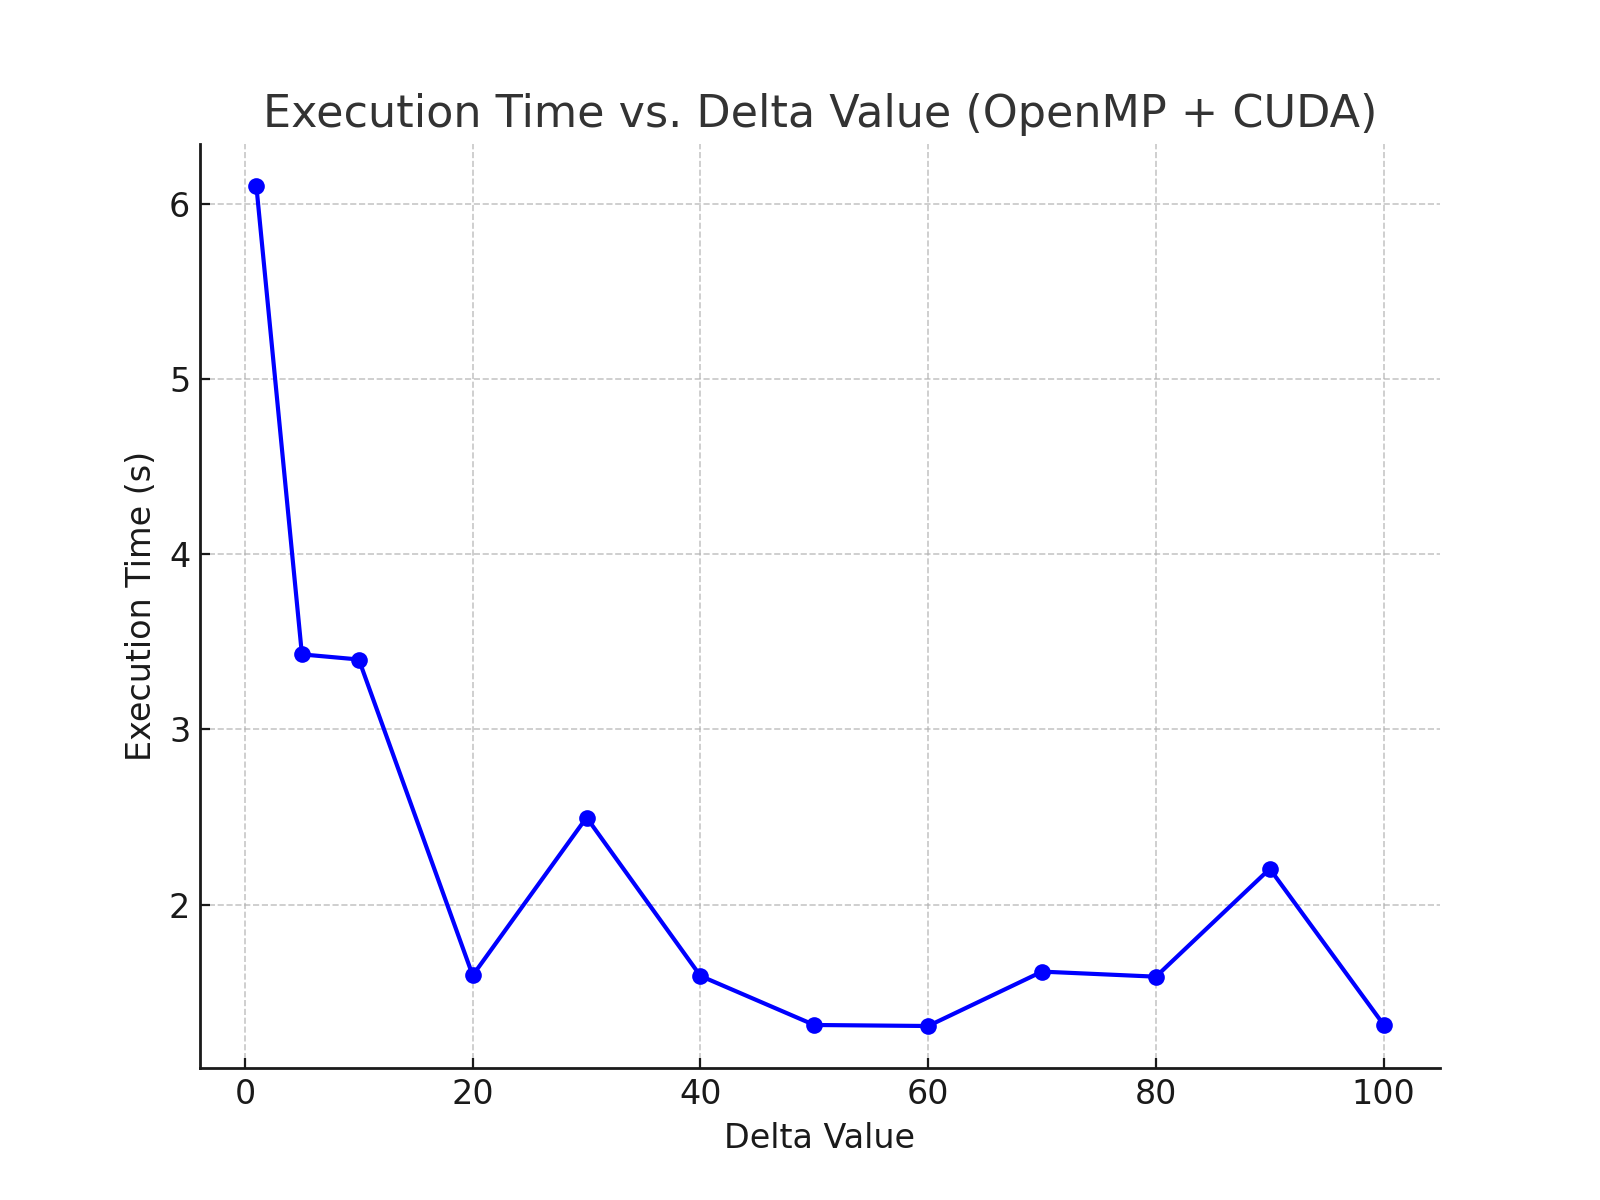
\includegraphics[width=0.4\textwidth]{execution_time_vs_delta.png}
    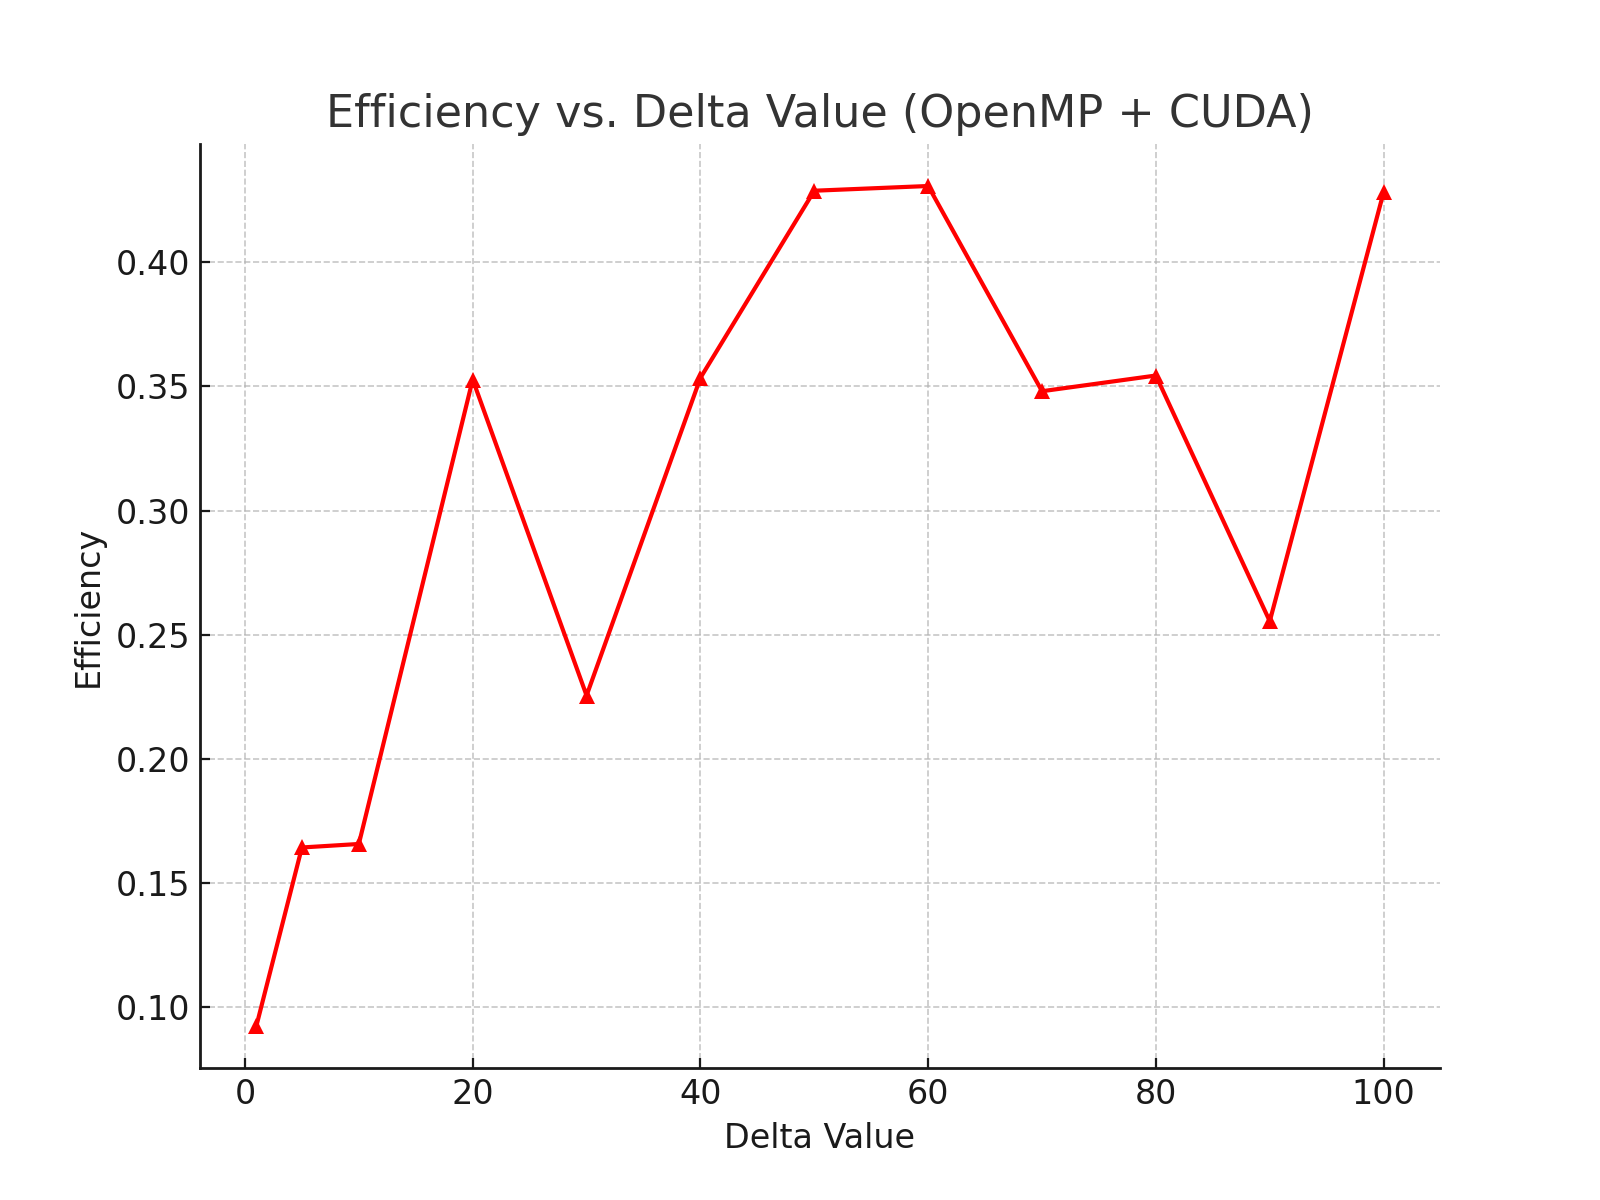
\includegraphics[width=0.4\textwidth]{efficiency_vs_delta.png}
    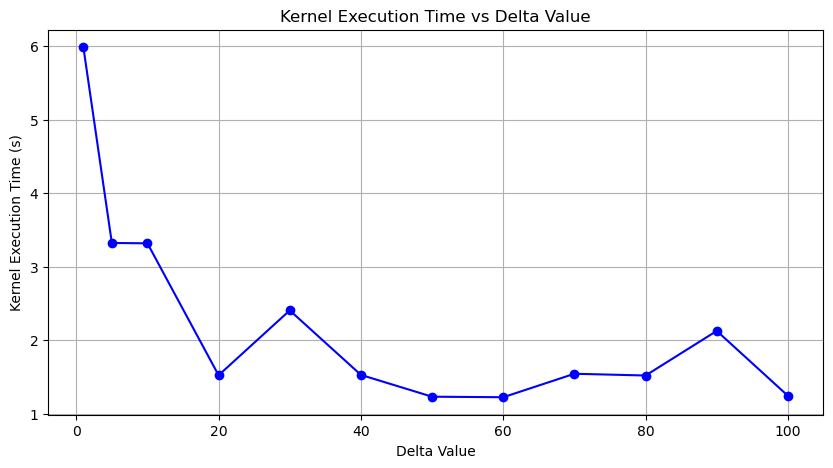
\includegraphics[width=0.4\textwidth]{KernelTime.png}
    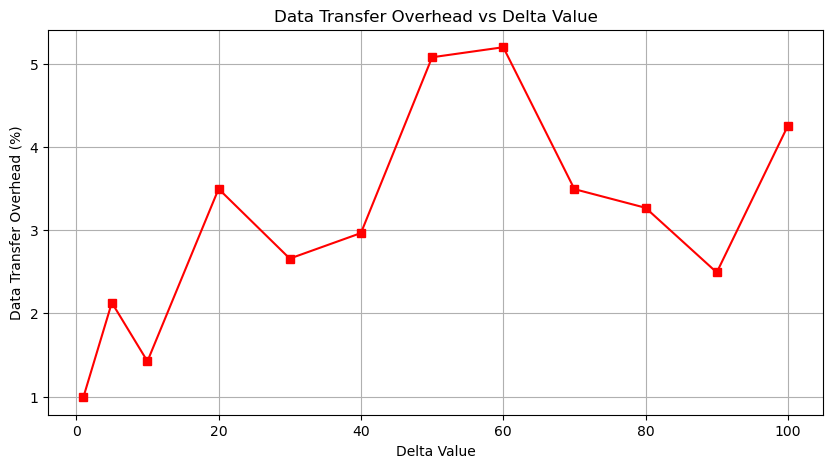
\includegraphics[width=0.4\textwidth]{kernelOverhead.png}

    \caption{Speedup vs Delta Values for OpenMP + CUDA Implementation}
    \label{fig:speedup_openmp_cuda}
\end{figure}

\section*{Results Analysis}

\subsection*{Effect of Delta Parameter on Performance}

The delta parameter in the Delta-Stepping algorithm determines bucket width and has a significant impact on performance. Our experiments with the hybrid OpenMP-CUDA implementation reveal several key insights about how varying delta affects different performance aspects.

\begin{figure}[ht]
    \centering
    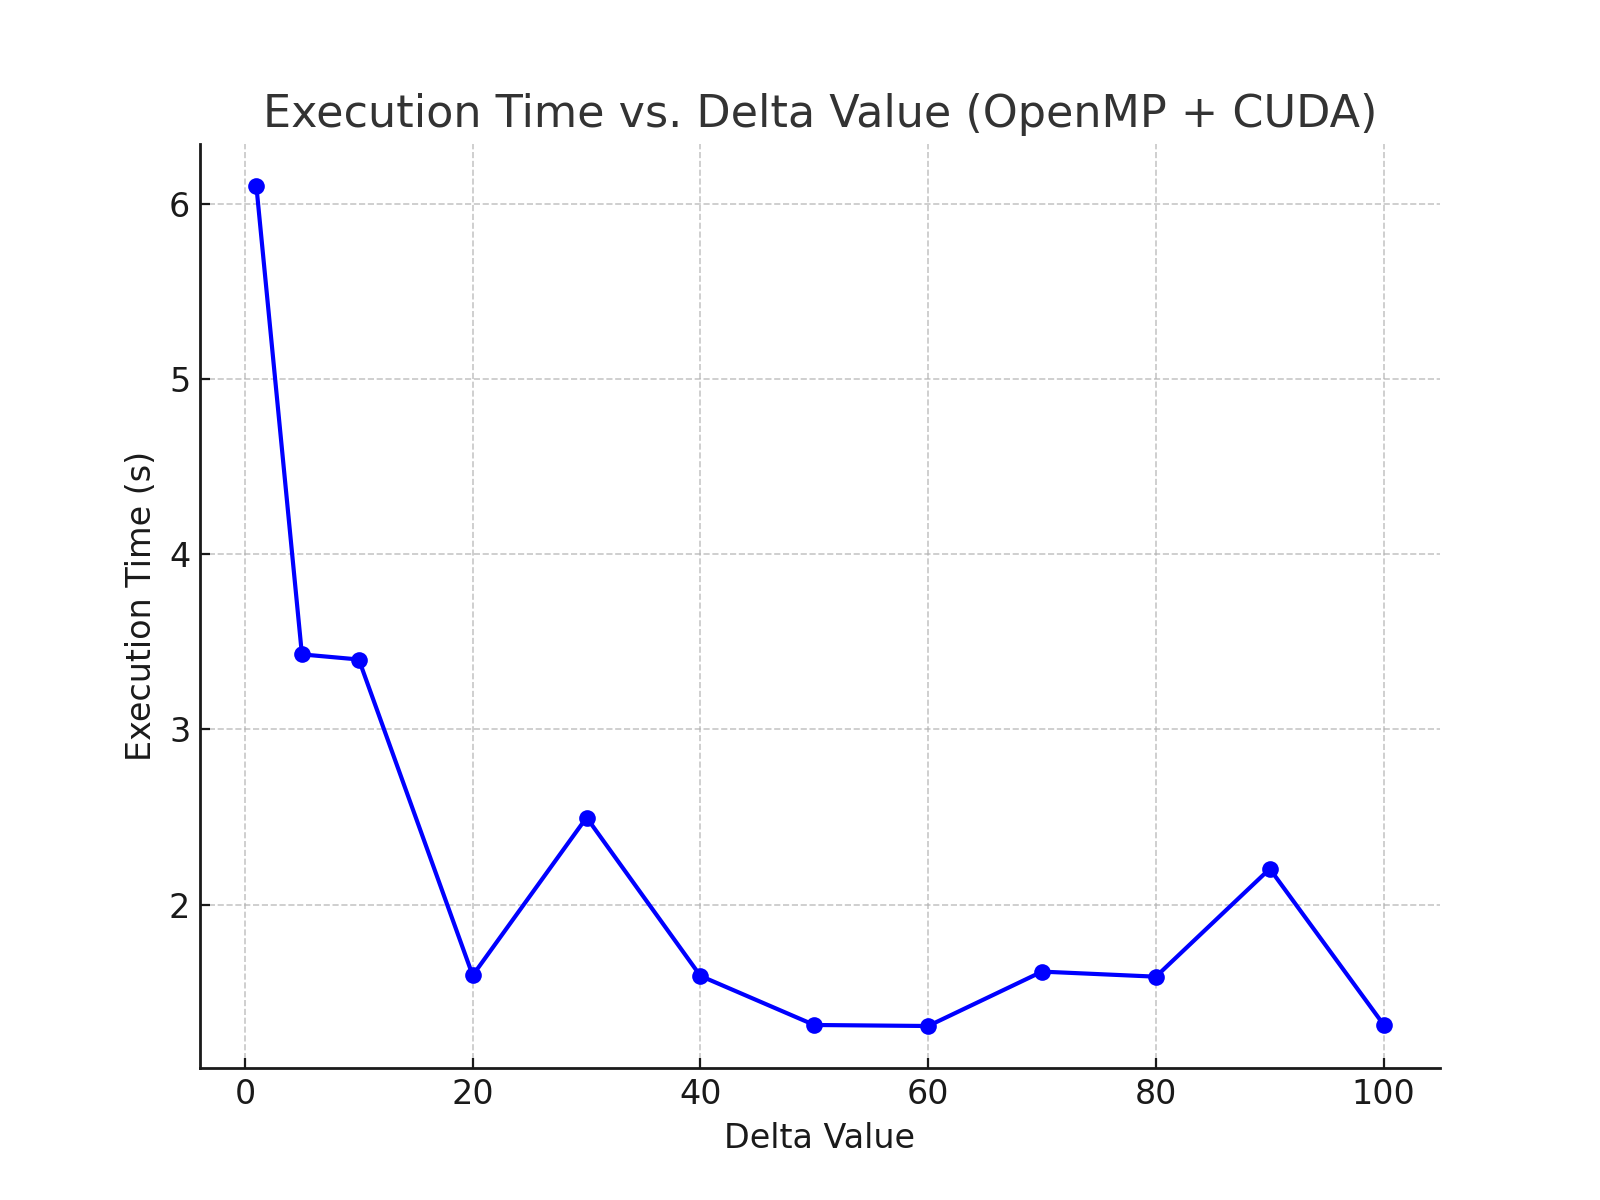
\includegraphics[width=\linewidth]{execution_time_vs_delta.png}
    \caption{Execution Time vs. Delta Value showing how bucket width affects overall performance}
    \label{fig:exec_time_delta}
\end{figure}

\subsubsection*{Execution Time Analysis}

Table~\ref{tab:delta_timing} and Figure~\ref{fig:exec_time_delta} show the relationship between delta values and execution time. Several observations can be made:

\begin{itemize}
    \item \textbf{Small Delta Values (1-10):} With small delta values, execution times are significantly higher (6.10s for $\delta=1$, 3.43s for $\delta=5$). This occurs because small buckets result in frequent GPU kernel launches and memory transfers, increasing overhead.
    
    \item \textbf{Medium Delta Values (50-60):} The optimal performance is achieved at $\delta=60$ with 1.31 seconds, representing a 3.44× speedup over sequential execution. This represents the sweet spot where buckets contain enough vertices to fully utilize GPU parallelism without excessive bucket management overhead.
    
    \item \textbf{Non-Monotonic Behavior:} Interestingly, the relationship is not monotonic. Performance decreases at $\delta=30$ (2.50s) and $\delta=90$ (2.20s), showing that the relationship between delta and performance is complex and depends on the graph structure.
\end{itemize}

\begin{figure}[ht]
    \centering
    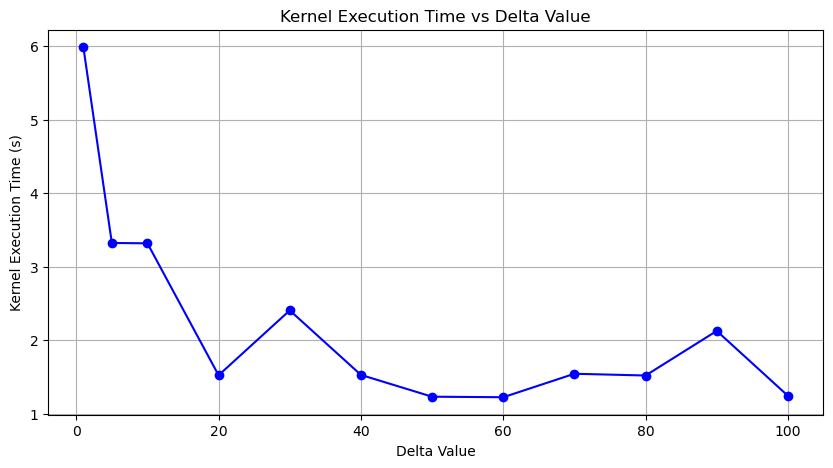
\includegraphics[width=\linewidth]{KernelTime.png}
    \caption{Kernel Execution Time vs. Delta Value showing GPU processing time for different bucket widths}
    \label{fig:kernel_time}
\end{figure}

\subsubsection*{Kernel Execution Time}

As shown in Figure~\ref{fig:kernel_time}, kernel execution time generally decreases as delta increases, with some exceptions:

\begin{itemize}
    \item At $\delta=1$, kernel execution time peaks at approximately 6 seconds due to a large number of small buckets requiring many kernel invocations.
    
    \item Performance improves significantly until $\delta=20$, then follows a pattern similar to overall execution time.
    
    \item The relationship between kernel time and delta exhibits local minima at $\delta=60$ and $\delta=100$, suggesting these values create efficiently sized work units for the GPU.
\end{itemize}

\begin{figure}[ht]
    \centering
    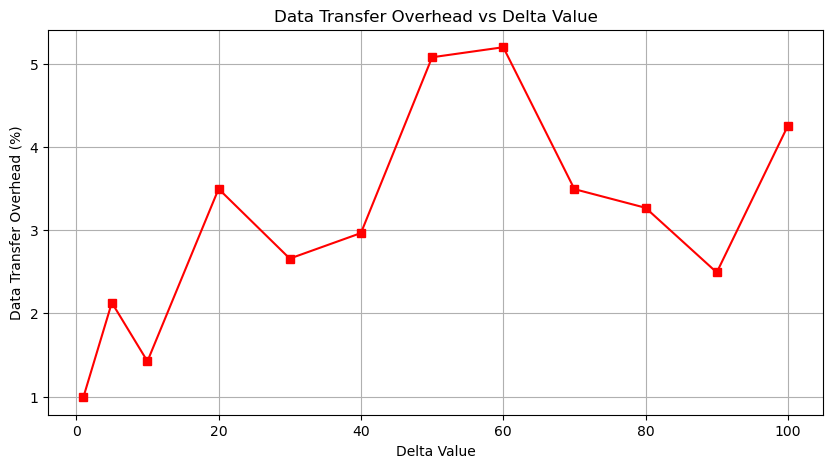
\includegraphics[width=\linewidth]{kernelOverhead.png}
    \caption{Data Transfer Overhead vs. Delta Value showing communication costs as percentage of total time}
    \label{fig:data_transfer}
\end{figure}

\subsubsection*{Data Transfer Overhead}

Figure~\ref{fig:data_transfer} shows the data transfer overhead as a percentage of total execution time:

\begin{itemize}
    \item Data transfer overhead is lowest at $\delta=1$ (approximately 1\%), as each bucket contains fewer vertices requiring less data transfer.
    
    \item The overhead peaks at approximately 5\% for $\delta=50$ and $\delta=60$, when larger buckets require more data to be transferred between CPU and GPU.
    
    \item The fluctuating pattern suggests that data transfer overhead is influenced by both bucket size and the number of iterations required for convergence.
\end{itemize}

\subsection*{Parallel Performance Metrics}

\begin{figure}[ht]
    \centering
    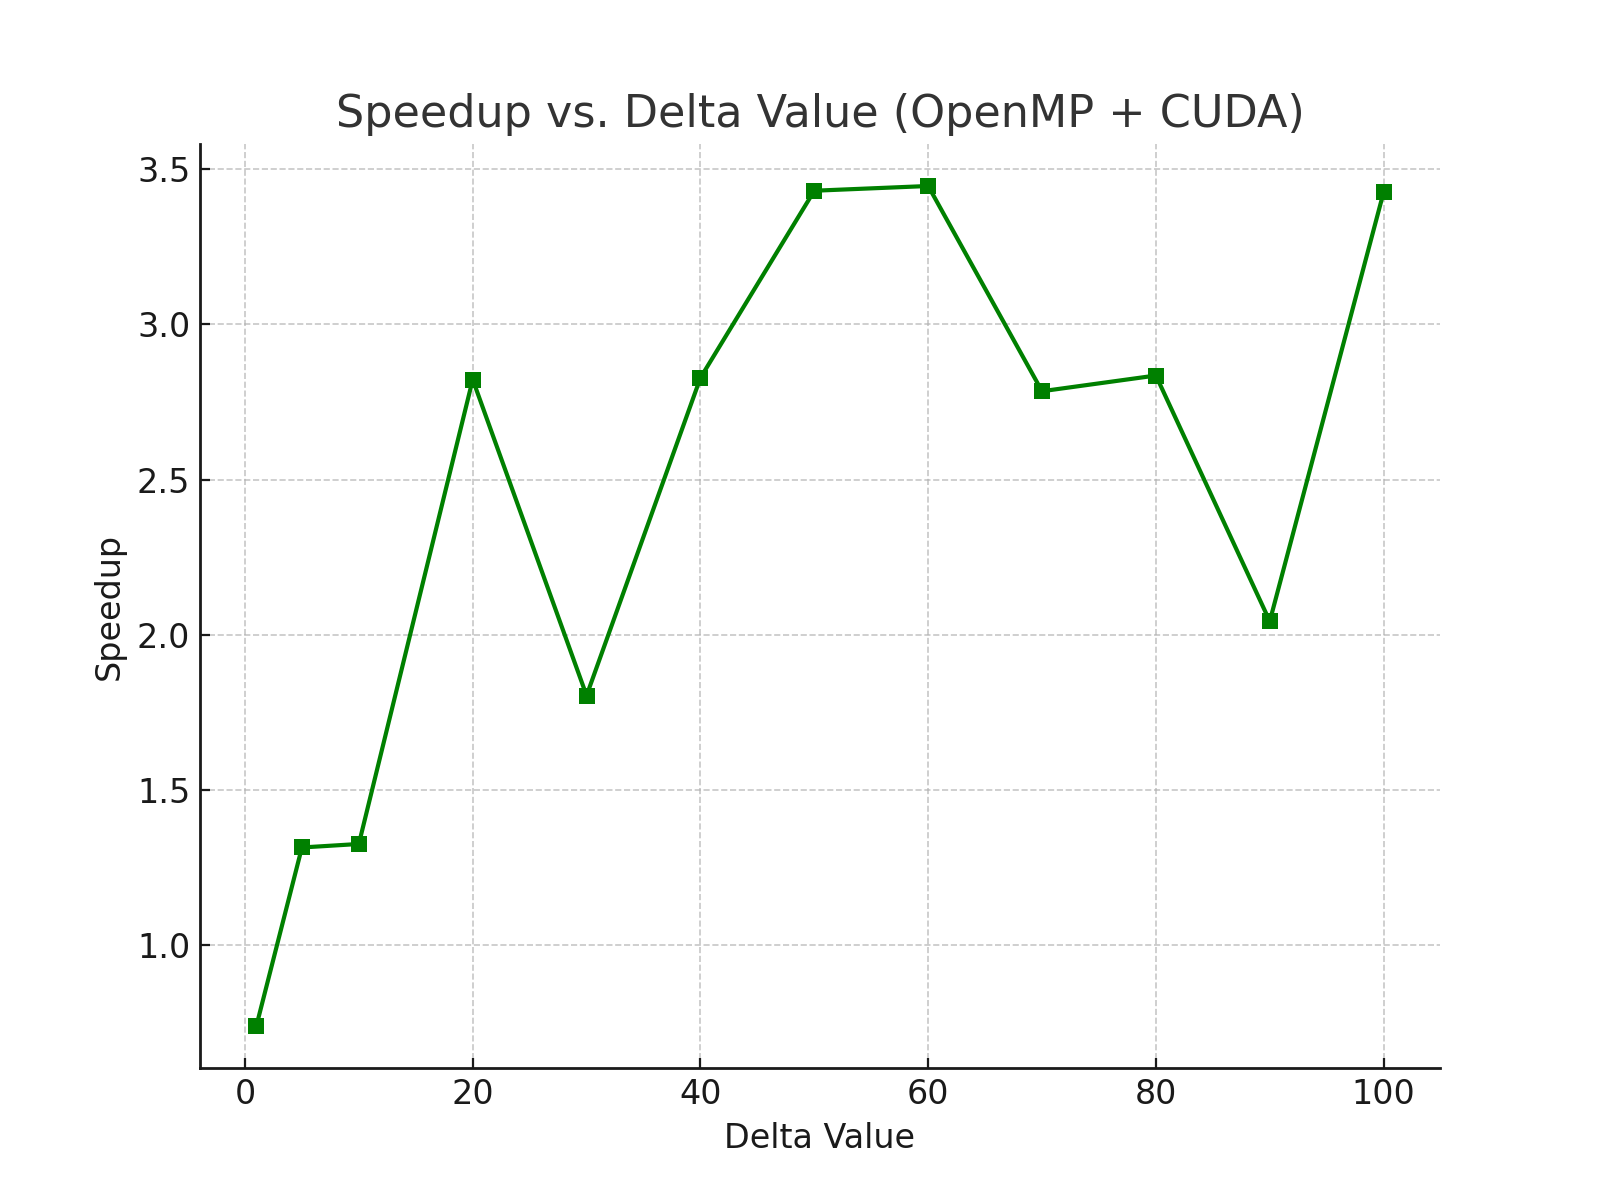
\includegraphics[width=\linewidth]{speedup_vs_delta.png}
    \caption{Speedup vs. Delta Value showing performance improvement relative to sequential algorithm}
    \label{fig:speedup_delta}
\end{figure}

\subsubsection*{Speedup Analysis}

Figure~\ref{fig:speedup_delta} illustrates the speedup achieved by our hybrid implementation compared to sequential Dijkstra's algorithm:

\begin{itemize}
    \item Speedup improves dramatically from $\delta=1$ (0.74×) to $\delta=60$ (3.44×), representing a 4.6× improvement in parallel performance through delta tuning alone.
    
    \item Maximum speedup of 3.44× is achieved at $\delta=60$, with similar performance at $\delta=100$ (3.43×).
    
    \item The speedup curve closely mirrors the inverse of execution time, confirming that delta tuning directly impacts parallel efficiency.
\end{itemize}

\begin{figure}[ht]
    \centering
    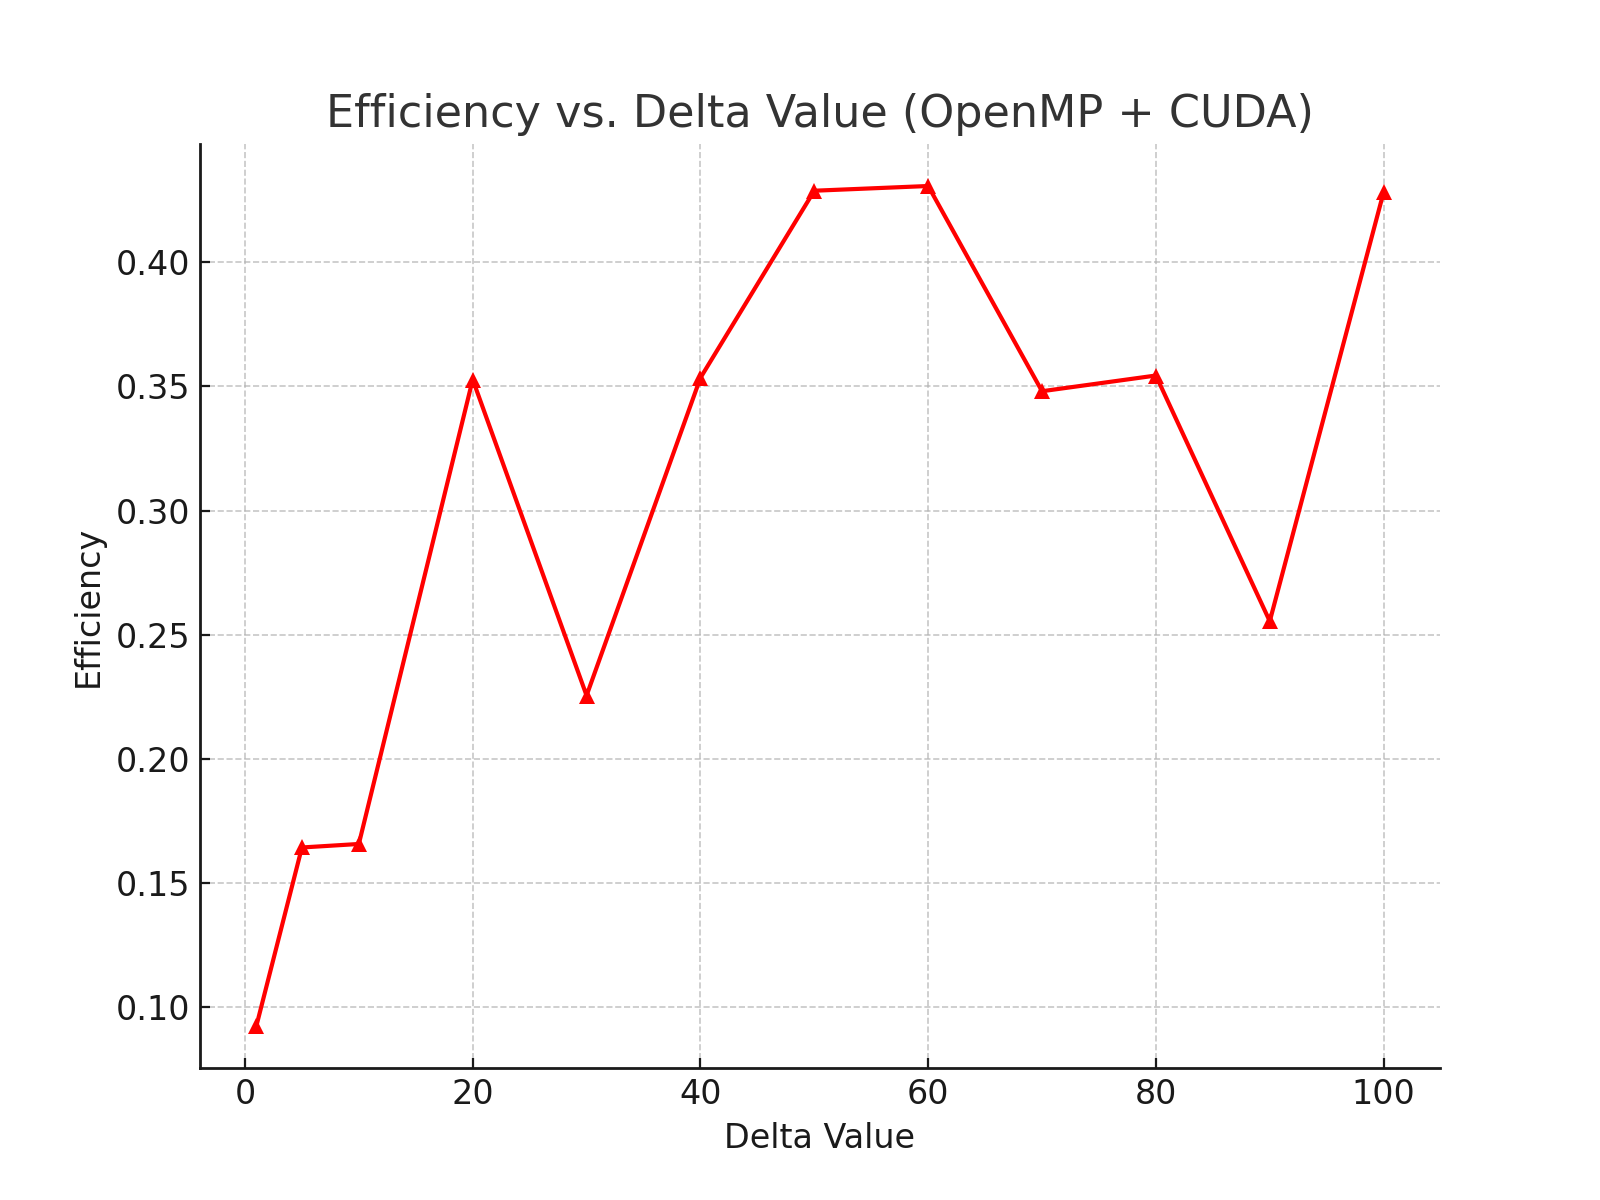
\includegraphics[width=\linewidth]{efficiency_vs_delta.png}
    \caption{Efficiency vs. Delta Value showing how effectively system resources are utilized}
    \label{fig:efficiency_delta}
\end{figure}

\subsubsection*{Efficiency Analysis}

Figure~\ref{fig:efficiency_delta} shows the parallel efficiency (speedup divided by processor count):

\begin{itemize}
    
    \item Efficiency at $\delta=1$ is only 9\%, demonstrating the critical importance of delta tuning for efficient resource utilization.
    
    \item The efficiency curve shows that delta values between 50 and 60 offer the best resource utilization for our test graph.
\end{itemize}

\begin{table}[ht]
    \centering
    \caption{Execution Times for Different Delta Values (OpenMP + CUDA)}
    \begin{tabular}{|c|c|}
        \hline
        \textbf{Delta Value} & \textbf{Execution Time (s)} \\
        \hline
        1 & 6.1021 \\
        \hline
        5 & 3.4281 \\
        \hline
        10 & 3.3989 \\
        \hline
        20 & 1.5955 \\
        \hline
        30 & 2.4969 \\
        \hline
        40 & 1.5924 \\
        \hline
        50 & 1.3124 \\
        \hline
        60 & 1.3066 \\
        \hline
        70 & 1.61707 \\
        \hline
        80 & 1.5882 \\
        \hline
        90 & 2.2041 \\
        \hline
        100 & 1.3141 \\
        \hline
    \end{tabular}
    \label{tab:delta_timing}

    Assuming Sequential Execution Time (T\_seq): 4.503 seconds
    \begin{equation}
        \text{Speedup} = \frac{T_{seq}}{T_{par}}
    \end{equation}
    and 
    \begin{equation}
        \text{Efficiency} = \frac{\text{Speedup}}{P}
    \end{equation}
    Where $T_{par}$ is the execution time for parallel implementation and $P$ is the number of processors which is 8 in this case.
\end{table}

\subsection*{Performance Bottleneck Analysis}

By comparing kernel execution time against data transfer overhead across different delta values, we can identify key performance bottlenecks:

\begin{itemize}
    \item For small delta values ($\delta < 20$), performance is primarily limited by \textbf{excessive kernel launches} and \textbf{serialization} due to small bucket sizes, even though data transfer overhead is minimal.
    
    \item For medium delta values ($40 \leq \delta \leq 60$), performance is optimal despite increased data transfer overhead, as efficient GPU utilization compensates for the increased communication costs.
    
    \item For certain delta values (notably $\delta=30$ and $\delta=90$), performance anomalies occur that correlate with the specific graph structure, suggesting that these values create particularly inefficient bucket distributions for the test graph.
\end{itemize}

\subsection*{Practical Implications}

Our experimental results lead to several practical recommendations for implementing hybrid CPU-GPU Delta-Stepping:

\begin{itemize}
    \item \textbf{Delta Parameter Selection:} For graphs similar to our test case, setting $\delta$ between 50 and 60 provides optimal performance. For other graphs, delta should be tuned based on average edge weight distribution.
    
    \item \textbf{Memory Transfer Optimization:} While memory transfers contribute to overhead, they do not dominate performance (max 5\% overhead), suggesting that our hybrid design effectively balances computation and communication.
    
    \item \textbf{Scalability:} The achieved efficiency of 43\% with 8 CPU threads indicates good scalability potential, though further optimizations in bucket management could improve this further.
\end{itemize}

\section*{Conclusion}

The experimental results demonstrate that our hybrid OpenMP-CUDA implementation of the Delta-Stepping algorithm achieves significant speedups compared to sequential execution, with performance heavily dependent on the delta parameter. The optimal delta value of 60 achieves a 3.44× speedup and 43\% efficiency on an 32-core system, confirming the effectiveness of the GPU-accelerated edge relaxation combined with CPU-based bucket management.

The non-monotonic relationship between delta and performance highlights the complexity of parallel shortest path algorithms, where work distribution, communication patterns, and graph characteristics all interact to determine overall efficiency. Our analysis provides valuable insights for tuning delta-stepping implementations on heterogeneous computing platforms, demonstrating that careful parameter selection can lead to substantial performance gains.


\end{document}
